\section{Schedule}{\label{secSched}}

The Project and Operations teams will complete several reviews as described below in order to closeout the construction phase, handover to Operations, and demonstrate readiness to begin the LSST. The first of these, Construction Completeness Review (CCR) 1, was held in October, 2024. CCR2 took place in July, 2025. Concurrent to CCR2, the Operations team went through the Operations Readiness Review (ORR) 1. Both reviews were run in parallel with the same NSF--DOE review panel convened to review and report out for the Observatory as a whole. A modest set of recommendations were made and Construction and Operations are addressing them. 

Construction Closeout and Operations Readiness Reviews:

\begin{itemize}
\item CCR1 -- readiness for the start of on-sky commissioning, as exemplified by substantial completion and integration of subsystems, and evidenced by direct measurement of the optical throughput of the integrated system

\item CCR2 -- capability to support LSST science goals, as exemplified by the System First Light technical milestone, and evidenced by delivered single-visit image quality (including active control of optics)

\item CCR3 -- reliability to initiate the LSST survey, as exemplified by the Science Validation Surveys, and evidenced by the readiness of Rubin Observatory Operations to accept the as-built Observatory

\item CCR4 -- closeout of the Construction project, as exemplified by service of scientifically validated survey-scale data products as part of the Operations Early Science Program, and evidenced by completed scope of system-level requirement verification, reporting, and final accounting
\end{itemize}

As of September 2025, the science validation phase of Construction is nearly complete. SV and system optimization will run through September 22. The facility will then shut down until October 24 to complete the remaining large integration activities that are required before starting regular operations. It is known that a number of activities will continue in operations managed by the construction project. These activities are captured in the "punch list". It is expected approximately 10 FTE of effort in FY26 going through at least June will be required to finish the punch list. 

CCR3/ORR2 will be held in October at the end of the observatory shut down. The combined review will be held with Observatory, partner, and agency staff. No review panel will be present. The team will present the status of the observatory following SV and the shutdown activity, the plans for the punch list, and the plans for early operations regarding continued optimization and readiness to start the LSST.

Following CCR3/ORR2 and the concurrent "Handover", the Operations team will begin to regularly run the system, taking responsibility for the observatory on October 25th. The priority for the Operations team is to drive the system to the state captured by the criteria in this document and start the LSST. Figure~\ref{sched} shows the current milestones for the Project and Operations. The period after CCR3/ORR2 is uncertain, but likely will involve continued pre--survey optimization. 

\begin{figure}%[]
  \centering
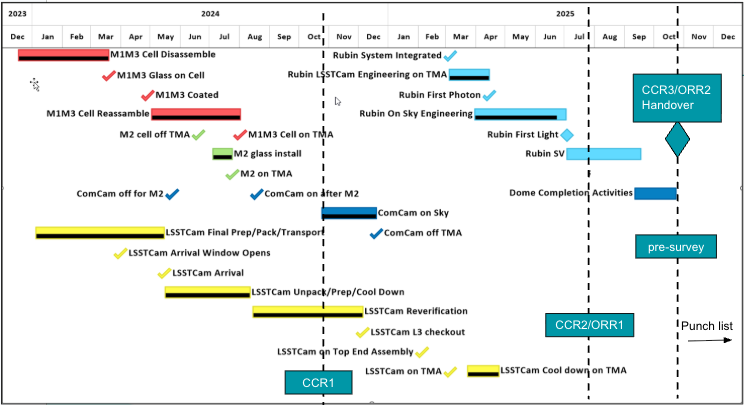
\includegraphics[width=0.95\linewidth]{sched.png}
\caption{Rubin Observatory Schedule as of September 01, 2025. Formal completeness reviews including operations readiness are shown in the Figure and described above. Handover to the Operations is set for October 25, 2025 and pre-survey optimization will continue until the performance criteria described in this document are met for starting the LSST. In parallel, some activities and work by the Construction team will continue in FY26. Some of these activities will positively impact on sky performance. }
\label{sched}
\end{figure}

\newpage
